% Options for packages loaded elsewhere
\PassOptionsToPackage{unicode}{hyperref}
\PassOptionsToPackage{hyphens}{url}
\PassOptionsToPackage{dvipsnames,svgnames,x11names}{xcolor}
%
\documentclass[
  letterpaper,
  DIV=11,
  numbers=noendperiod]{scrartcl}

\usepackage{amsmath,amssymb}
\usepackage{iftex}
\ifPDFTeX
  \usepackage[T1]{fontenc}
  \usepackage[utf8]{inputenc}
  \usepackage{textcomp} % provide euro and other symbols
\else % if luatex or xetex
  \usepackage{unicode-math}
  \defaultfontfeatures{Scale=MatchLowercase}
  \defaultfontfeatures[\rmfamily]{Ligatures=TeX,Scale=1}
\fi
\usepackage{lmodern}
\ifPDFTeX\else  
    % xetex/luatex font selection
\fi
% Use upquote if available, for straight quotes in verbatim environments
\IfFileExists{upquote.sty}{\usepackage{upquote}}{}
\IfFileExists{microtype.sty}{% use microtype if available
  \usepackage[]{microtype}
  \UseMicrotypeSet[protrusion]{basicmath} % disable protrusion for tt fonts
}{}
\makeatletter
\@ifundefined{KOMAClassName}{% if non-KOMA class
  \IfFileExists{parskip.sty}{%
    \usepackage{parskip}
  }{% else
    \setlength{\parindent}{0pt}
    \setlength{\parskip}{6pt plus 2pt minus 1pt}}
}{% if KOMA class
  \KOMAoptions{parskip=half}}
\makeatother
\usepackage{xcolor}
\setlength{\emergencystretch}{3em} % prevent overfull lines
\setcounter{secnumdepth}{-\maxdimen} % remove section numbering
% Make \paragraph and \subparagraph free-standing
\makeatletter
\ifx\paragraph\undefined\else
  \let\oldparagraph\paragraph
  \renewcommand{\paragraph}{
    \@ifstar
      \xxxParagraphStar
      \xxxParagraphNoStar
  }
  \newcommand{\xxxParagraphStar}[1]{\oldparagraph*{#1}\mbox{}}
  \newcommand{\xxxParagraphNoStar}[1]{\oldparagraph{#1}\mbox{}}
\fi
\ifx\subparagraph\undefined\else
  \let\oldsubparagraph\subparagraph
  \renewcommand{\subparagraph}{
    \@ifstar
      \xxxSubParagraphStar
      \xxxSubParagraphNoStar
  }
  \newcommand{\xxxSubParagraphStar}[1]{\oldsubparagraph*{#1}\mbox{}}
  \newcommand{\xxxSubParagraphNoStar}[1]{\oldsubparagraph{#1}\mbox{}}
\fi
\makeatother


\providecommand{\tightlist}{%
  \setlength{\itemsep}{0pt}\setlength{\parskip}{0pt}}\usepackage{longtable,booktabs,array}
\usepackage{calc} % for calculating minipage widths
% Correct order of tables after \paragraph or \subparagraph
\usepackage{etoolbox}
\makeatletter
\patchcmd\longtable{\par}{\if@noskipsec\mbox{}\fi\par}{}{}
\makeatother
% Allow footnotes in longtable head/foot
\IfFileExists{footnotehyper.sty}{\usepackage{footnotehyper}}{\usepackage{footnote}}
\makesavenoteenv{longtable}
\usepackage{graphicx}
\makeatletter
\newsavebox\pandoc@box
\newcommand*\pandocbounded[1]{% scales image to fit in text height/width
  \sbox\pandoc@box{#1}%
  \Gscale@div\@tempa{\textheight}{\dimexpr\ht\pandoc@box+\dp\pandoc@box\relax}%
  \Gscale@div\@tempb{\linewidth}{\wd\pandoc@box}%
  \ifdim\@tempb\p@<\@tempa\p@\let\@tempa\@tempb\fi% select the smaller of both
  \ifdim\@tempa\p@<\p@\scalebox{\@tempa}{\usebox\pandoc@box}%
  \else\usebox{\pandoc@box}%
  \fi%
}
% Set default figure placement to htbp
\def\fps@figure{htbp}
\makeatother

\KOMAoption{captions}{tableheading}
\makeatletter
\@ifpackageloaded{tcolorbox}{}{\usepackage[skins,breakable]{tcolorbox}}
\@ifpackageloaded{fontawesome5}{}{\usepackage{fontawesome5}}
\definecolor{quarto-callout-color}{HTML}{909090}
\definecolor{quarto-callout-note-color}{HTML}{0758E5}
\definecolor{quarto-callout-important-color}{HTML}{CC1914}
\definecolor{quarto-callout-warning-color}{HTML}{EB9113}
\definecolor{quarto-callout-tip-color}{HTML}{00A047}
\definecolor{quarto-callout-caution-color}{HTML}{FC5300}
\definecolor{quarto-callout-color-frame}{HTML}{acacac}
\definecolor{quarto-callout-note-color-frame}{HTML}{4582ec}
\definecolor{quarto-callout-important-color-frame}{HTML}{d9534f}
\definecolor{quarto-callout-warning-color-frame}{HTML}{f0ad4e}
\definecolor{quarto-callout-tip-color-frame}{HTML}{02b875}
\definecolor{quarto-callout-caution-color-frame}{HTML}{fd7e14}
\makeatother
\makeatletter
\@ifpackageloaded{caption}{}{\usepackage{caption}}
\AtBeginDocument{%
\ifdefined\contentsname
  \renewcommand*\contentsname{Table of contents}
\else
  \newcommand\contentsname{Table of contents}
\fi
\ifdefined\listfigurename
  \renewcommand*\listfigurename{List of Figures}
\else
  \newcommand\listfigurename{List of Figures}
\fi
\ifdefined\listtablename
  \renewcommand*\listtablename{List of Tables}
\else
  \newcommand\listtablename{List of Tables}
\fi
\ifdefined\figurename
  \renewcommand*\figurename{Figure}
\else
  \newcommand\figurename{Figure}
\fi
\ifdefined\tablename
  \renewcommand*\tablename{Table}
\else
  \newcommand\tablename{Table}
\fi
}
\@ifpackageloaded{float}{}{\usepackage{float}}
\floatstyle{ruled}
\@ifundefined{c@chapter}{\newfloat{codelisting}{h}{lop}}{\newfloat{codelisting}{h}{lop}[chapter]}
\floatname{codelisting}{Listing}
\newcommand*\listoflistings{\listof{codelisting}{List of Listings}}
\makeatother
\makeatletter
\makeatother
\makeatletter
\@ifpackageloaded{caption}{}{\usepackage{caption}}
\@ifpackageloaded{subcaption}{}{\usepackage{subcaption}}
\makeatother

\usepackage{bookmark}

\IfFileExists{xurl.sty}{\usepackage{xurl}}{} % add URL line breaks if available
\urlstyle{same} % disable monospaced font for URLs
\hypersetup{
  pdftitle={Module 1: Logic and the language of mathematics},
  pdfauthor={Nathan Alexander, PhD},
  colorlinks=true,
  linkcolor={blue},
  filecolor={Maroon},
  citecolor={Blue},
  urlcolor={Blue},
  pdfcreator={LaTeX via pandoc}}


\title{Module 1: Logic and the language of mathematics}
\usepackage{etoolbox}
\makeatletter
\providecommand{\subtitle}[1]{% add subtitle to \maketitle
  \apptocmd{\@title}{\par {\large #1 \par}}{}{}
}
\makeatother
\subtitle{EDUC 315 - Howard University}
\author{Nathan Alexander, PhD}
\date{}

\begin{document}
\maketitle


\section{Module overview}\label{module-overview}

This module provides an overview of fundamental concepts in number,
logic, and mathematical reasoning. We'll explore the principles of
deductive and inductive reasoning, and begin to develop a foundation for
understanding logical arguments and mathematical proofs.

We'll also explore concepts such as quantity, structure, space, and
change, which form the basis of the various mathematical disciplines.
Special attention is given to the concepts of zero and infinity, their
historical development, and their significance in mathematical thinking.

\section{Notes}\label{notes}

\subsection{The concept of sets}\label{the-concept-of-sets}

A set is a well-defined collection of distinct objects. A set is
considered as an object in its own right. Sets are foundational in
mathematics because they provide a way to group and classify numbers,
objects, or ideas. The items inside a set are called the set's elements.

\begin{tcolorbox}[enhanced jigsaw, leftrule=.75mm, colframe=quarto-callout-tip-color-frame, opacitybacktitle=0.6, breakable, opacityback=0, colbacktitle=quarto-callout-tip-color!10!white, bottomrule=.15mm, arc=.35mm, colback=white, toprule=.15mm, rightrule=.15mm, left=2mm, bottomtitle=1mm, title=\textcolor{quarto-callout-tip-color}{\faLightbulb}\hspace{0.5em}{Elements}, toptitle=1mm, coltitle=black, titlerule=0mm]

An element is an object or item in a set.

For example, for \(A = \{1, 3, 5\} \text{ and } B = \{2, 4, 6\}\), we
say \(3 \in A\) and \(4 \in B\).

\end{tcolorbox}

If an element \(a\) is in set \(A\), we write \(a \in A\).

If a is not in \(A\), we write \(a \notin A\).

\begin{center}\rule{0.5\linewidth}{0.5pt}\end{center}

\begin{tcolorbox}[enhanced jigsaw, leftrule=.75mm, colframe=quarto-callout-tip-color-frame, opacitybacktitle=0.6, breakable, opacityback=0, colbacktitle=quarto-callout-tip-color!10!white, bottomrule=.15mm, arc=.35mm, colback=white, toprule=.15mm, rightrule=.15mm, left=2mm, bottomtitle=1mm, title=\textcolor{quarto-callout-tip-color}{\faLightbulb}\hspace{0.5em}{Membership}, toptitle=1mm, coltitle=black, titlerule=0mm]

The fundamental property of sets is that elements are either members or
non-members -- there is no in-between. The symbol \(\in\) (epsilon) is
used to denote membership.

\end{tcolorbox}

In this context, \(\in\) (epsilon) means: ``is an element of,'' ``is a
member of,'' or simply ``is in.''

To indicate non-membership, we use \(\notin\).

For example, for the same set \(A = \{1, 3, 5\}\), we write
\(6 \notin A\).

\begin{center}\rule{0.5\linewidth}{0.5pt}\end{center}

\begin{tcolorbox}[enhanced jigsaw, leftrule=.75mm, colframe=quarto-callout-tip-color-frame, opacitybacktitle=0.6, breakable, opacityback=0, colbacktitle=quarto-callout-tip-color!10!white, bottomrule=.15mm, arc=.35mm, colback=white, toprule=.15mm, rightrule=.15mm, left=2mm, bottomtitle=1mm, title=\textcolor{quarto-callout-tip-color}{\faLightbulb}\hspace{0.5em}{Subsets}, toptitle=1mm, coltitle=black, titlerule=0mm]

A set \(A\) is a subset of \(B\) if every element of \(A\) is also in
\(B\).

We write \(A \subseteq B\) to indicate subsets.

\end{tcolorbox}

\begin{center}\rule{0.5\linewidth}{0.5pt}\end{center}

\begin{tcolorbox}[enhanced jigsaw, leftrule=.75mm, colframe=quarto-callout-tip-color-frame, opacitybacktitle=0.6, breakable, opacityback=0, colbacktitle=quarto-callout-tip-color!10!white, bottomrule=.15mm, arc=.35mm, colback=white, toprule=.15mm, rightrule=.15mm, left=2mm, bottomtitle=1mm, title=\textcolor{quarto-callout-tip-color}{\faLightbulb}\hspace{0.5em}{Operations}, toptitle=1mm, coltitle=black, titlerule=0mm]

\paragraph{Union}\label{union}

The \textbf{union} of sets \(A\) and \(B\) is the set of all elements in
\(A\) or \(B\):

\[
A \cup B = \{ x \mid x \in A \text{ or } x \in B \}
\]

\paragraph{Intersection}\label{intersection}

The \textbf{intersection} of sets \(A\) and \(B\) is the set of all
elements in both \(A\) and \(B\):

\[
A \cap B = \{ x \mid x \in A \text{ and } x \in B \}
\]

\paragraph{Complement}\label{complement}

The \textbf{complement} of set \(A\) (relative to a universal set \(U\))
is the set of all elements in \(U\) not in \(A\):\\
\[
A^{c} = \{ x \in U \mid x \notin A \}
\]

\end{tcolorbox}

\begin{center}\rule{0.5\linewidth}{0.5pt}\end{center}

\subsection{Sets of numbers}\label{sets-of-numbers}

\begin{center}\rule{0.5\linewidth}{0.5pt}\end{center}

\subsubsection{Natural numbers}\label{natural-numbers}

The set of \textbf{natural} numbers, \(\mathbb{N} = \{1, 2, 3, ...\}\)

\subsubsection{Whole numbers}\label{whole-numbers}

The set of \textbf{whole} numbers,
\(\mathbb{N_0} = \{0, 1, 2, 3, ...\}\)

\subsubsection{Integer numbers}\label{integer-numbers}

The set of \textbf{integers},
\(\mathbb{Z} = \{..., -3, -2, -1, 0, 1, 2, 3, ...\}\)

\subsubsection{Rational numbers}\label{rational-numbers}

The set of \textbf{rational} numbers,
\(\mathbb{Q} = \{\dfrac{a}{b}, a \in \mathbb{Z}, b \in \mathbb{Z}, b \ne 0\}\)

\subsubsection{Real numbers}\label{real-numbers}

\begin{itemize}
\tightlist
\item
  The set of \textbf{real} numbers, \(\mathbb{R} = (-\infty, \infty)\)
\end{itemize}

\begin{center}\rule{0.5\linewidth}{0.5pt}\end{center}

\subsubsection{Other sets}\label{other-sets}

What sets are missing? How can you define and visualize these other
sets?

\begin{figure}[H]

{\centering \pandocbounded{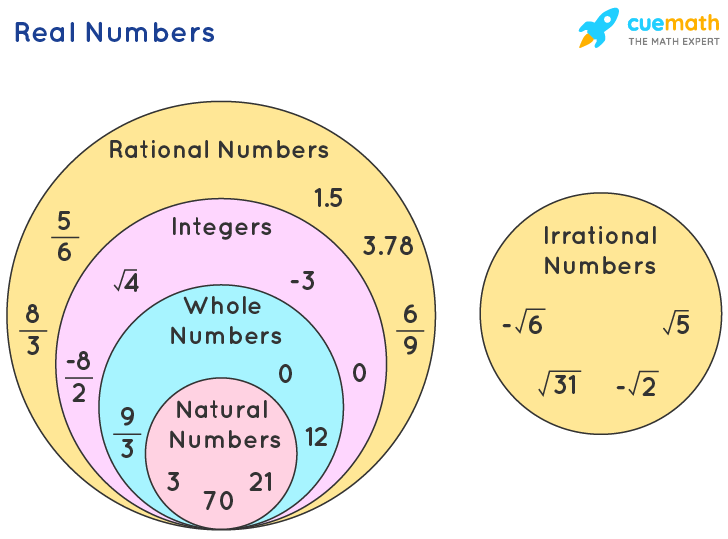
\includegraphics[keepaspectratio]{module01_files/mediabag/real-numbers-1-16215.png}}

}

\caption{Sets of numbers. From cuemath.com}

\end{figure}%

\begin{center}\rule{0.5\linewidth}{0.5pt}\end{center}

\subsection{Framing mathematics and
science}\label{framing-mathematics-and-science}

\textbf{Science} is the systematic study and pursuit of knowledge about
the natural and physical world through observation, experimentation, and
the formulation of testable hypotheses. It involves a methods-based
approach to understanding phenomena and developing explanations based on
empirical evidence. \textbf{Mathematics} is the science that deals with
the logic of quantity, structure, space, and change.

\begin{center}\rule{0.5\linewidth}{0.5pt}\end{center}

\subsubsection{Logic}\label{logic}

Logic refers to the principles of reasoning, especially correct
reasoning. It's the systematic method of coming to conclusions through
rational thought. In mathematics, logic involves the formal principles
of reasoning and inference used to derive valid conclusions.

\begin{center}\rule{0.5\linewidth}{0.5pt}\end{center}

\subsubsection{Reasoning}\label{reasoning}

\begin{itemize}
\item
  \textbf{Deductive reasoning}: Deductive reasoning is a logical process
  that involves drawing specific conclusions from general premises or
  principles that are assumed to be true. This form of reasoning is
  often described as a ``top-down'' approach, where one starts with a
  general statement and applies it to a specific case. In mathematics,
  deductive reasoning involves using established rules, facts, and
  theorems to draw specific conclusions. It moves from general
  principles to specific instances.

  \begin{itemize}
  \item
    For example, if we know that ``All fish live in water'' and ``Nemo
    is a fish,'' what can we conclude?
  \item
    Solving equations: Rule: If (x + 5 = 12), you can subtract (5) from
    both sides. Specific case: Your equation is (x + 5 = 12).
    Conclusion: (x = 7).
  \item
    Even numbers: Rule: All even numbers can be divided by (2) with no
    remainder. Specific case: (48) is an even number. Conclusion: (48)
    can be divided by (2) with no remainder.
  \end{itemize}
\end{itemize}

\begin{center}\rule{0.5\linewidth}{0.5pt}\end{center}

\subsubsection{Reasoning}\label{reasoning-1}

\begin{itemize}
\item
  \textbf{Inductive reasoning}: Inductive reasoning is a logical process
  that involves drawing general conclusions from specific observations
  or instances. This method is often referred to as ``bottom-up''
  reasoning, contrasting with deductive reasoning, which moves from
  general principles to specific conclusions. In mathematics, inductive
  reasoning involves observing patterns or specific instances to form
  general conclusions or hypotheses.

  \begin{itemize}
  \item
    Number patterns: You see the sequence (2, 4, 6, 8, \dots) You notice
    each number adds (2). You guess that the next number is (10).
  \item
    You multiply (3 \times 5 = 15), then (7 \times 9 = 63). Both answers
    are odd. You guess that multiplying any two odd numbers always gives
    an odd number.
  \item
    More generally, using if-then statements.
  \end{itemize}
\end{itemize}

\begin{center}\rule{0.5\linewidth}{0.5pt}\end{center}

\subsubsection{Quantity}\label{quantity}

Quantity relates to the amount or number of something that can be
measured or counted. In mathematics, it deals with concepts like
magnitude, size, or amount that can be expressed numerically.

\begin{figure}[H]

{\centering \pandocbounded{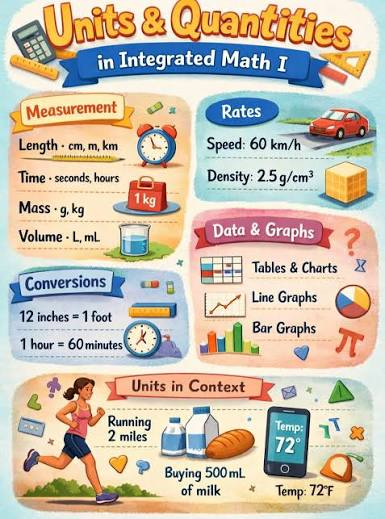
\includegraphics[keepaspectratio]{../img/quantity.jpg}}

}

\caption{Sample quantities}

\end{figure}%

\begin{center}\rule{0.5\linewidth}{0.5pt}\end{center}

\subsubsection{Structure}\label{structure}

Structure in mathematics refers to the way mathematical objects are
organized or arranged.

\begin{figure}[H]

{\centering \pandocbounded{
\includegraphics[keepaspectratio]{../img/structure.gif}}

}

\caption{Structure of mathematics}

\end{figure}%

Structure involves the relationships and patterns between mathematical
entities, such as the properties of number systems or the organization
of geometric shapes.

\begin{center}\rule{0.5\linewidth}{0.5pt}\end{center}

\subsubsection{Space}\label{space}

In mathematics, space refers to the framework within which points,
lines, shapes, and other geometric objects exist.

\begin{figure}[H]

{\centering \pandocbounded{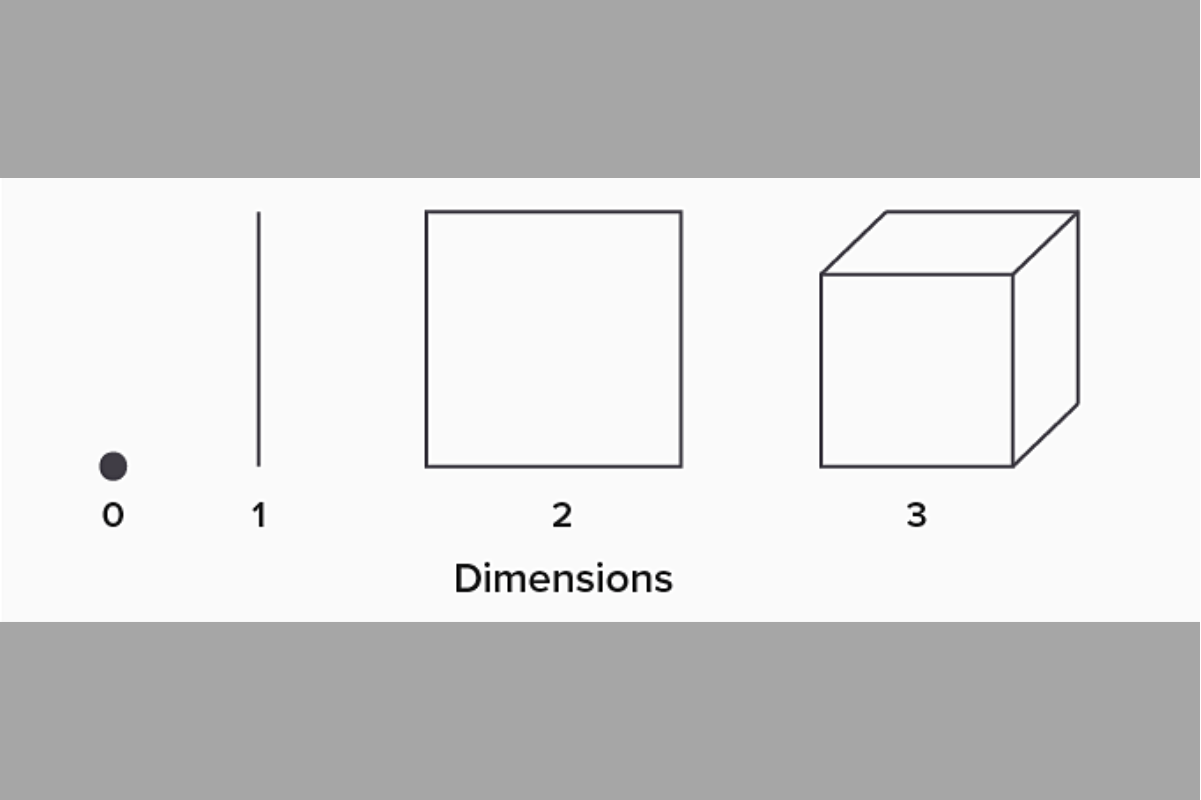
\includegraphics[keepaspectratio]{../img/space.png}}

}

\caption{Dimensions in space}

\end{figure}%

Space can be two-dimensional (like a plane), three-dimensional (like our
physical world), or even higher-dimensional in abstract mathematics.

\begin{center}\rule{0.5\linewidth}{0.5pt}\end{center}

\subsubsection{Change}\label{change}

Change in mathematics deals with how quantities or properties vary or
transform over time or under different conditions. This concept is
fundamental to areas like calculus, which studies rates of change and
accumulation.

\begin{figure}[H]

{\centering \pandocbounded{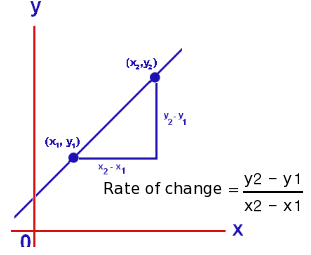
\includegraphics[keepaspectratio]{../img/rate-of-change.png}}

}

\caption{Rate of change}

\end{figure}%

\section{What do we mean by zero?}\label{what-do-we-mean-by-zero}

Zero is a number that represents the absence of quantity or magnitude.
It is the integer between the set of all negative integers and all
positive integers.

\subsection{Examples}\label{examples}

The empty set: \(\emptyset\) or \(\{ \}\).

The number line: A starting point on number line.

Counting: of you have a basket of apples and remove all of the apples,
you are left with zero apples.

Temperature: On the Celsius scale, zero degrees represents the freezing
point of water.

\section{What do we mean by
infinity?}\label{what-do-we-mean-by-infinity}

Infinity is a concept describing something without any limit, and is
larger than any real number. It is often denoted by the symbol
\(\infty\).

\subsection{Examples}\label{examples-1}

The number line: You can always add 1 to any number, no matter how
large, so the number line extends infinitely.

Fractional division: 1 divided by 3 results in a repeating decimal
(0.333\ldots) that goes on infinitely.

\begin{center}\rule{0.5\linewidth}{0.5pt}\end{center}

\subsection{Key points to remember:}\label{key-points-to-remember}

\begin{itemize}
\item
  Zero as a placeholder in our number system.
\item
  The role of zero in mathematics (e.g., additive identity).
\item
  Historical developments of the concept of zero:

  \begin{itemize}
  \item
    Dividing a number by zero, \(\dfrac{x}{0} = \text{undefined}\) for
    some number \(x \neq 0\)
  \item
    Dividing zero by zero, \(\dfrac{x}{0} = \text{undefined}\) for some
    number \(x = 0\).
  \end{itemize}
\item
  Different types of infinity (countable and uncountable)
\item
  The concept of infinity in mathematics vs.~everyday life
\item
  Paradoxes involving infinity (e.g., Hilbert's Hotel)
\end{itemize}

\begin{center}\rule{0.5\linewidth}{0.5pt}\end{center}

\subsection{Hilbert's Hotel}\label{hilberts-hotel}

\emph{How the Paradox Works}

Imagine a hotel with a countable infinity of rooms: 1, 2, 3, 4, and so
on, with no last room.

Every single room is already full.

In a normal hotel, you cannot take new guests when every room is full.

\pandocbounded{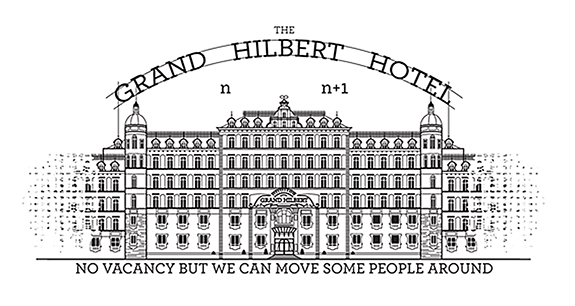
\includegraphics[keepaspectratio]{../img/hilberts-hotel.png}}

\emph{Adding a Single New Guest}

A new traveler arrives and wants a room.

The manager asks the guest in room 1 to move to room 2.

The guest in room 2 moves to room 3, and every guest \(n\) moves to room
\(n + 1\).

Room 1 is now empty for the new traveler, and nobody is left without a
room.

This proves that infinity plus one is still just infinity.




\end{document}
